\documentclass[article,slovene]{stucosrec}

% for testing purposes only
\usepackage{lipsum}

% Example of defining a new command
\newcommand{\latex}{\LaTeX\xspace}
\newcommand{\bibtex}{Bib\TeX\xspace}
\newcommand{\stucosrec}{StuCoSReC\xspace}
\newcommand{\latexe}{\LaTeX$2_\epsilon$\xspace}

\title{\latex predloga za prispevke StuCoSReC}
\author{
	Klemen Berkovič\thanks{Če ima ta avtor več e-poštnih naslovov, jih lahko dodate tukaj. Na primer: email1@email.com, email2@email.si} \\
	Fakulteta za elektotehniko, \\računalništvo in informatiko,\\
	Univerza v Mariboru,\\
	Koro\v{s}ka cesta 46, 2000 Maribor, Slovenija \\
	\texttt{klemen.berkovic1@um.si}
	\And
	Iztok Fister Jr.\thanks{Če ima ta avtor več pridruženih univerz, jih lahko dodate tukaj. Če obstaja več dopisnih avtorjev, to povejte v tem poglavju.} \\
	Fakulteta za elektotehniko, \\računalništvo in informatiko,\\
	Univerza v Mariboru,\\
	Koro\v{s}ka cesta 46, 2000 Maribor, Slovenija \\
	\texttt{iztok.fister1@um.si}
	\AND
	Iztok Fister \thanks{Če ima ta avtor telefonsko številko, jo lahko dodate tukaj. Telefonska številka mora vsebovati klicno kodo države. Na primer: +xx-xxxx-xxx-xxxx} \\
	Fakulteta za elektotehniko, \\računalništvo in informatiko,\\
	Univerza v Mariboru,\\
	Koro\v{s}ka cesta 46, 2000 Maribor, Slovenija \\
	\texttt{iztok.fister@um.si}
}

% images directory
\imagespath{ {./images/} }

\begin{document}
	
	\maketitle
	
	\begin{abstract}
        Ta dokument predstavlja šablono dokumenta \latex, ki ustreza stilskim smernicam konferenčnega zbornika \stucosrec in služi kot vodič k pripravi prispevka za to konferenco s pomočjo \latexe in \bibtex.
        Ta izvorna koda je bila napisana z namenom prevajanja z \latexe in \bibtex.
        Avtorji so poskušali zajeti vse možne posebnosti, kot so podnaslovi, opombe naslovov, podnaslovov, avtorjev ter besedila in vse izbirne komponente (npr. pregledi, dodatni avtorji, reference, zahvale) ter primere enačb, tabel, slik, seznamov in algoritmov.
        Za najboljši izkoristek tega dokumenta ga poženite z \latex in \bibtex in primerjate izhod tega dokumenta z izhodom vašega dokumenta.
    \end{abstract}
	
	% keywords can be removed
	\keywords{\stucosrec zbornik \and \latex \and označevanje besedila\footnote{Navedite tri do deset ključnih besed specifičnih vašemu prispevku, vendar vseeno pogosto uporabljenih znotraj vaše discipline.}}
	
	
    \section{Uvod}
	
	V \textit{zborniku} so trajno zbrani prispevki predstavljeni na konferenci \stucosrec.
	Organizacijski odbor te konference se trudi, da so ti prispevki uniformni in kakovostni, zato ima nekaj strogih pravil za formatiranje prispevkov. 
	Predpisan je dvovrstični format, font (Arial, Helvetica ali Times Roman) in njegova velikost (na primer 11pt za telo), predpisana je tudi velikost robov (1,76cm na vrhu, 2,54cm na dnu in 1,6cm na straneh), širina stolpca (8,71cm) in razmaka med stolpcema (0,35cm).

	Za vse našteto na srečo poskrbi pripravljen razred \latex.
	Dodatno mora avtor uporabiti možnost \textbf{article} v ponujenem razredu dokumenta (ang. \textit{``document class''}) za ustvarjanje članka.
	Če želi avtor ustvariti povzetek, mora uporabiti možnost \textbf{abstract} namesto \textbf{article}.
	Oddani članki, ki so delo raziskav študentov, se recenzirajo.
	Članek je lahko v slovenskem jeziku, za katerega je potrebno dodati možnost \textbf{slovene} k razredu dokumenta.
	Članki morajo vsebovati dovolj podrobnosti, da lahko programski odbor oceni njihovo kvaliteto.
	V postopku pošiljanja dokumenta v recenzijski postopek mora avtor dodati možnost \textbf{review} k razredu dokumenta. Ko je članek sprejet, mora avtor odstraniti možnost \textbf{review}.
	Članki so omejeni na največ \textbf{štiri strani} v \texttt{pdf} formatu.

	Preostanek tega dokumenta služi kot prikaz specifičnih ukazov \latex v kontekstu dejanskih primerov, ne pa natančnemu opisu in razlagi teh ukazov.
	
	\section{\textit{Jedro} članka}
	
	Običajno je jedro članka organizirano v hierarhično strukturo z oštevilčenimi ali neoštevilčenimi naslovi, podnaslovi in podpodnaslovi poglavij ter manjših odsekov.
	Ukaz \texttt{{\char'134}section} pred tem odstavkom je del take hierarhije\footnote{Ukaza {\texttt{\char'134 And}} in/ali {\texttt{\char'134 AND}} ste že uporabili pri umeščanju avtorjev članka.}. \latex sam, ob uporabi ustreznih ukazov za naslove, ureja oštevilčevanje in umestitev teh naslovov.
	Če želite, da je podnaslov neoštevilčen, preprosto dodajte zvezdico k imenu ukaza.
	Primeri oštevilčenih in neoštevilčenih naslovov se bodo pojavili tekom tega dokumenta\footnote{To je druga opomba. Ne podaja nobene pomembne informacije, temveč služi samo prikazu, kako delujejo in izgledajo opombe. Ta je precej dolga zato, da vidite, kako se takšna dolga opomba prikaže v končnem dokumentu.}.
	
	Ker je celoten članek v okolju \textbf{document}, lahko začetek novega odstavka označite z prazno vrstico. Zato je ta stavek v novem odstavku.
	
	\subsection{Spremembe pisave in \textit{posebni} znaki}
	
	V tem dokumentu smo videli že nekaj sprememb pisave.
	V vašem tekstu lahko besede ali besedne zveze naredite ležeče z uporabo ukaza \texttt{{\char'134}textit}, krepke z uporabo ukaza \texttt{{\char'134}textbf} in v stilu pisalnega stroja (na primer za programsko kodo) z ukazom \texttt{{\char'134}texttt}.
	Ne pozabite, da za spremembe pisave, ki so del \textit{strukturnih elementov} (kot so na primer naslovi poglavij), poskrbi podana datoteka razreda dokumenta. Bodite previdni pri uporabi zavitih oklepajev pri spreminjanju pisave, saj le-ti določajo začetek in konec besedila, ki ga želite v drugi pisavi.
	
	Znotraj vašega dokumenta lahko uporabljate poljubne simbole, posebne znake ali tuje znake\footnote{Tretja opomba. Ta je precej kratka.}. Seznam vseh razpoložljivih simbolov najdete v \textit{\latex User's Guide}~\cite{Lamport:LaTeX}.
	
	\subsection{Matematične enačbe}
	
	Matematične enačbe lahko prikažete v treh različnih slogih: vrstni (ang. \textit{Inline}), oštevilčen ali neštevilčen blokovni prikaz.
	V naslednjih poglavjih obravnavamo vse naštete sloge podrobneje.
	
	\subsubsection{Vrstne enačbe}
	
	Enačba, ki se pojavi znotraj vrstice besedila, se imenuje vrstna enačba.
	Doseže se z uporabo okolja \textbf{math}, ki ga lahko prikličete z običajnimi \texttt{{\char'134}begin {\char'134}end} ukazi, ali krajše z \textbf{\$$\cdots$\$}.
	Uporabite lahko katerekoli simbole in strukture, od $\alpha$ do $\omega$, ki so na voljo v \latex~\cite{Lamport:LaTeX}. Ta odsek bo prikazal nekaj preprostih primerov vrstnih enačb.
	Opazite, kako prikazana vrstna enačba:
	\begin{math}\lim_{n\rightarrow \infty}x=0\end{math}, 
	izgleda nekoliko drugače kot prikazana v blokovnem prikazu (glej naslednje poglavje).

	
	\subsubsection{Blokovne enačbe}
	
	Oštevilčeno blokovno enačbo -- takšno, ki je navpično odmaknjena od besedila in vodoravno poravnana -- kreiramo z uporabo okolja \textbf{equation}.
	Neoštevilčene blokovne enačbe vpeljemo z uporabo okolja \textbf{displaymath}.

	Ponovno lahko v obeh okoljih uporabljate poljubne simbole in strukture, ki so na voljo v \latex. Ta odsek prikazuje nekaj primerov blokovnih enačb.
	Najprej poglejmo enačbo, ki je bila prej prikazana v vrstnem načinu: 
	\begin{equation}\lim_{n\rightarrow \infty}x=0.\end{equation}
	Opazite, kako je v okolju \textbf{displaymath} izgled drugačnejši od vrstnega prikaza.
	Vzemimo, pa primer, neštevilčeno enačbo:
	\begin{displaymath}\sum_{i=0}^{\infty} x + 1\end{displaymath},
	ki ji sledi še številčena: 
	\begin{equation}\sum_{i=0}^{\infty}x_i=\int_{0}^{\pi+2} f\end{equation},
	da prikažemo možnost številčenja v \latex.
	
	Sledi primer neštevilčene enačbe, ki ni definirana v okolju \textbf{displaymath}, temveč v kratki obliki \textbf{\$\$$\cdots$\$\$}.
	Ko $a \ne 0$, obstajata dve rešitvi enačbe $ax^2 + bx + c = 0$, in sicer: $$x_{1, 2} = \frac{-b \pm \sqrt{b^2-4ac}}{2a}.$$
	
	Tukaj je primer sklicevanja na enačbo. Enačba~(\ref{equ:yannibel}) prikazuje, kako v \latex pisati pogoje.
	
	\begin{equation}
		\begin{aligned} 
			\mathrm{nr}(G_i,r) & = \label{equ:yannibel}
			\begin{cases}
				1  & \text{$r$ je igran z enim članom iz $G_i$}\\
				-2 & \text{$r$ ni igran s članom iz $G_i$} \\
				-p & \text{$r$ je igran s $p$ člani iz $G_i$}\\
			\end{cases}
		\end{aligned}
	\end{equation}

	\subsubsection{Dolge enačbe}
	
	Kadar je enačba predolga za en stolpec, uporabite okolje \textbf{aligned} znotraj okolja \textbf{equation}.
	Za poravnavo enačbe znotraj \textbf{aligned} okolja uporabite znak \textbf{\&}, kot je razvidno iz enačbe~(\ref{equ:ho}):
	
	\begin{equation}
		\begin{aligned}
			O_{\max}& = w_1 \sum_{a=1}^{m} \sum_{b=a+1}^{n} (-\lvert\text{CPT}_a 
			-\text{CPT}_b\rvert)\\ 
			&\quad + w_2 \sum_{j=1}^{m} (\text{DIF}_j) + w_3 \sum_{j=1}^{m} 
			(\text{INT}_j/\sum_{x=1}^{n} x_{ij})
		\end{aligned}
		\label{equ:ho}
	\end{equation}

    \subsection{Citiranje}
	
	Citati člankov \cite{lecun2015deep, braams:babel, herlihy:methodology}, konferenčnih zbornikov \cite{vrbancic2019transfer, clark:pct} ali knjig \cite{salas:calculus, Lamport:LaTeX, fister2019computational}, navedenih
	v bibliografijskem delu vašega članka, se bodo pojavili skozi celotno besedilo vašega članka.
	Za samodejno izdelavo te bibliografije uporabite \bibtex. Uporabiti morate samo enega izmed mnogih ukazov za citiranje, s ključem vira, ki ga želite citirati, na ustreznem mestu znotraj \texttt{.tex} datoteke \cite{Lamport:LaTeX}.
	Ključ vira je kratka opomba, ki si jo določite sami tako, da enolično določa posamezen vir. V tem dokumentu za ključ uporabljamo avtorjev priimek in besedo z naslova vira.
	Ključ vira je definiran pri vsakem vnosu v \texttt{.bib} datoteko vašega članka.
	
	Podrobnosti ustvarjanja \texttt{.bib} datoteke so izven domene tega dokumenta, vendar lahko več informacij najdete v \textit{Author's Guide} in \textit{\latex User's Guide}\cite{Lamport:LaTeX}.

	Ta dokument prikazuje samo najosnovnejšo obliko ukaza za citiranje \texttt{{\char'134}cite}.
	Ta je določena v specifikacijah slogov ACM za citiranje.
	Drugi načini citiranja niso dovoljeni v predlogi.
	
	\subsection{Tabele}
	
	Ker tabel ni mogoče razdeliti na več strani, je zanje najboljša umestitev na vrhu ali dnu strani, najbližje prvemu sklicu na tabelo.
	Da zagotovite to pravilno umestitev in poravnavo tabel, uporabite okolje \textbf{table}, v katerega ovijete vsebino in naslov tabele.
	Sama vsebina tabele se mora nahajati znotraj okolja \textbf{tabular}, da je zagotovljena pravilna poravnava vrstic in stolpcev.
	Podrobnejša navodila so ponovno dostopna v \textit{\latex User's Guide}.
		
	Tabela~\ref{tab:table1} je vstavljena takoj za tem stavkom; primerjajte umestitev tabele znotraj izvorne datoteke z umestitvijo znotraj \texttt{pdf} izhoda te datoteke.
	
	\begin{table}
		\centering
		\caption{Frekvence posebnih znakov.}
		\label{tab:table1}
		\begin{tabular}{|c|c|l|} \hline
			Simbol&Frekvenca&Komentar\\ \hline
			\O & 1 na 1,000& Švedska imena.\\ \hline
			$\pi$ & 1 na 5& V matematiki.\\ \hline
			\$ & 4 na 5 & V ekonomiji.\\ \hline
			$\Psi^2_1$ & 1 na 40,000& Nepojasnjeno. \\ \hline
		\end{tabular}
	\end{table}

	Če želite širšo tabelo, ki zavzame celotno širino delovnega območja na strani, uporabite okolje \textbf{table*}, v katerega ovijete vsebino in naslov tabele.
	Kot pri tabeli z enim stolpcem, bo tudi ta samodejno umeščena na ustrezno mesto.
	Tabela~\ref{tab:table2} je vstavljena takoj za tem stavkom; ponovno primerjajte umestitev tabele znotraj izvorne datoteke z umestitvijo znotraj \texttt{pdf} izhoda te datoteke.
	
	\begin{table*}
		\centering
		\caption{Nekaj tipičnih ukazov.}
		\label{tab:table2}
		\begin{tabular}{|c|c|l|} \hline
			Ukaz&Numerična vresnost&Komentar\\ \hline
			\texttt{{\char'134}imagespath} & 200 & Mapa kjer se nahajajo slike dokumenta. \\ \hline
			\texttt{{\char'134}table} & 300 & Za tabele.\\ \hline
			\texttt{{\char'134}table*} & 400& Za široke tabele.\\ \hline
		\end{tabular}
	\end{table*}

	\subsection{Slike}
	
	Podobno kot tabele, se tudi slike ne morejo deliti na strani. Tudi zanje je najboljša umestitev na vrh ali dno strani, najbližje prvemu sklicu na sliko\footnote{Četrta, zadnja, opomba.}.
	Da zagotovite ustrezno umestitev, uporabite okolje \textbf{figure}, v katerega vnesete sliko in njen opis.
	
	Ta vzorčni dokument vsebuje primer prikaza \texttt{.pdf} datotek z \latex.
	Uporaba tega tipa datotek za prikaz je vidna na sliki~\ref{fig:circles}.
	
	\begin{figure}
		\centering
		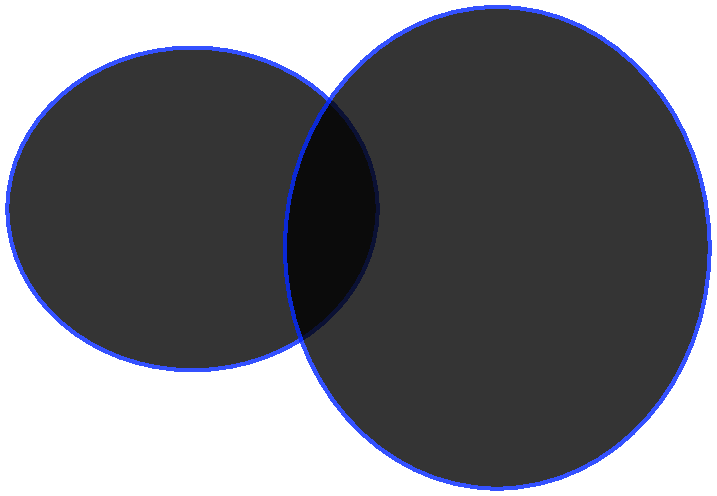
\includegraphics[scale=0.5]{circles.pdf}
		\caption{Vzorčna slika krogov (\texttt{.pdf} format).}
		\label{fig:circles}
	\end{figure}

	Ta vzorčni dokument vsebuje primer prikaza \texttt{.png} datotek z \latex.
	Uporaba tega tipa datotek za prikaz je vidna na sliki~\ref{fig:star}.
	
	\begin{figure}
		\centering
		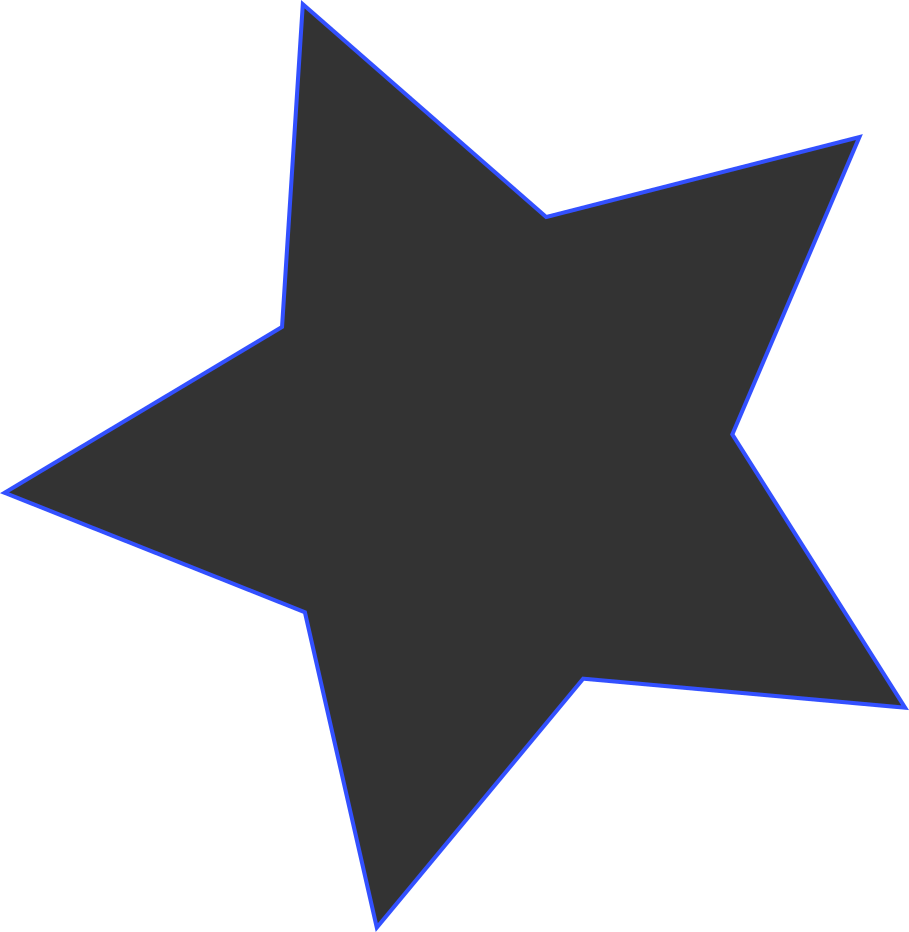
\includegraphics[scale=0.5]{star.png}
		\caption{Vzorčna slika zvezde (\texttt{.png} format).}
		\label{fig:star}
	\end{figure}

	Kakor pri tabelah, lahko tudi pri slikah uporabite širši prikaz, ki se razteza čez dva stolpca.
	Za dosego tega in zagotovitvijo ustrezne umestitve slike uporabite okolje \textbf{figure*}.
	Primer omenjenega je viden na sliki~\ref{fig:spin}.
	
	\begin{figure*}
		\centering
		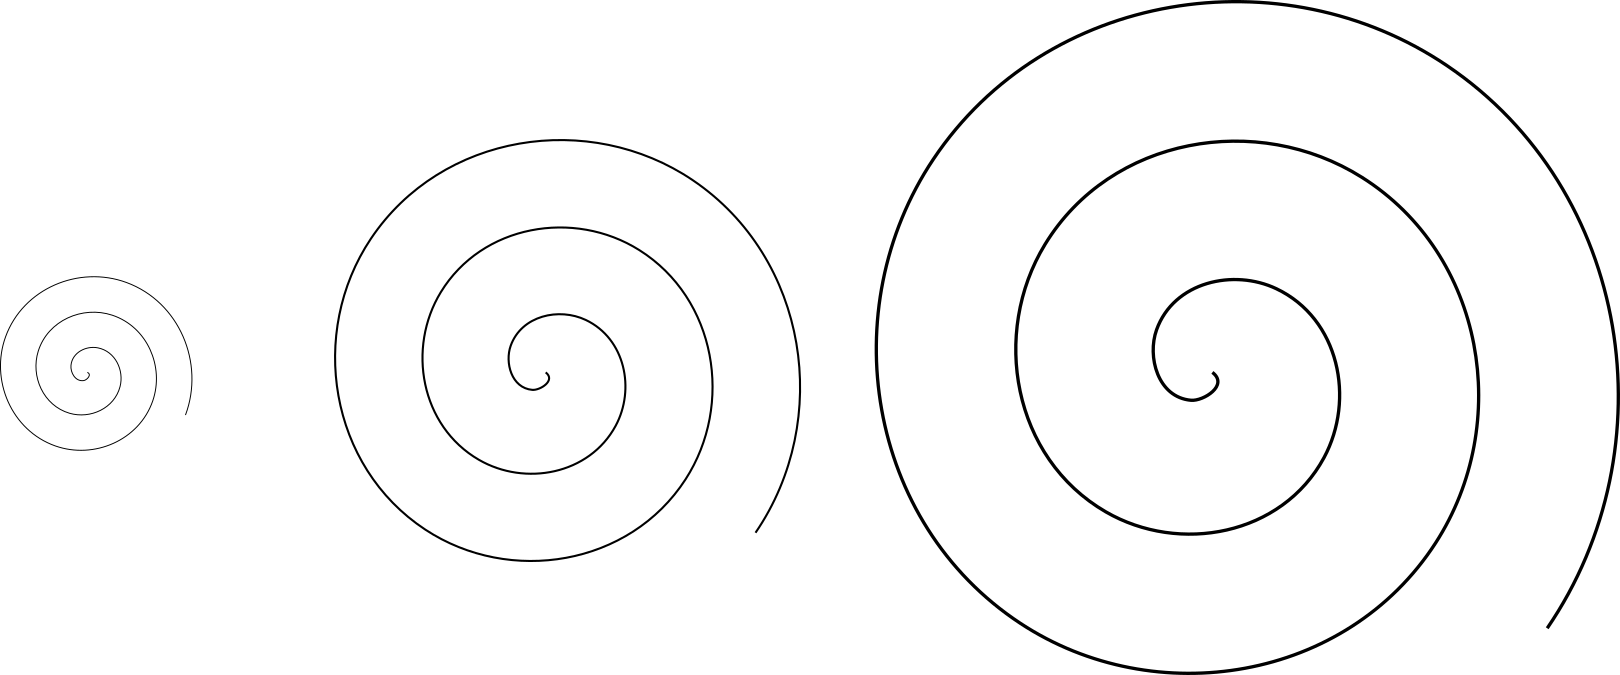
\includegraphics[scale=0.8]{spin.png}
		\caption{Primer preproste slike.}
		\label{fig:spin}
	\end{figure*}

	\subsection{Seznami}
	
	V dokumentu lahko uporabite sezname, da bralcu podate informacije v postavkah.
	Seznami se ustvarijo z uporabo okolja \textbf{itemize}.
	Naslednji seznam je primer ustvarjanja in uporabe seznama:
	
	\begin{itemize}
		\item prvi element,
		\item drugi element
		\item tretji element.
	\end{itemize}
	
	Včasih se avtorji želijo sklicevati na posamezne postavke seznama.
	Za dosego tega se lahko uporabi okolje \textbf{enumerate}.
	Primer oštevilčenega seznama:
	
	\begin{enumerate}
	    \item prva točka,
	    \item druga točka,
	    \item $\cdots$
	\end{enumerate}
	
	Ob sklicu na seznam se sedaj lahko sklicujemo tudi na posamezne postavke seznama.

	\subsection{Algoritmi}
	
	Če želite znotraj vašega prispevka vstaviti algoritem, preverite primer algoritma~\ref{algo:sample}.
	Algoritmi so zapisani znotraj okolja \textbf{algorithm}.
	
	\begin{algorithm}
		\SetAlgoLined
		\KwData{tukaj je tekst}
		\KwResult{kako pisati algoritme v \latexe}
		inicializacija\;
		\tcc{to je komentar ki sporoča začetek pomembne kode}
		\While{ni konec dokumenta}{\label{algo:sample:while}
			beri del dokumenta\;
			\eIf{razumeš}{
				pojdi v naslednjo sekcijo\;
				trenutna sekcija postane ta\;
			}{
				vrni se na začetek trenutne sekcije\;
			}
		}
		\caption{Kako pisati algoritme.}
		\label{algo:sample}
	\end{algorithm}

	Kot je razvidno iz naslednjega stavka, se lahko sklicujete tudi na posamezne vrstice algoritma, .
	Primer zanke \textbf{while} je viden v vrstici~\ref{algo:sample:while}.
	Podrobnejša navodila glede okolja \textbf{algorithm} lahko najdete v \url{http://tug.ctan.org/macros/latex/contrib/algorithm2e/doc/algorithm2e.pdf}.
	
	\section{Zaključek}
	
	Ta odstavek končuje jedro tega vzorčnega dokumenta.
	Ne pozabite, da morate dodati morda še zahvalo (kratek primer zahvale sledi v nadaljevanju).
	Dodatno morate še urediti bibliografijo, mi pa moramo povedati, da so sklici, z izjemo \latex knjige, znotraj tega dokumenta nepovezani s to temo in služijo zgolj kot primeri.
	
	\begin{acknowledgment}
		Ta razdelek ni obvezen; na tem mestu se lahko zahvalite za morebitna sredstva, financiranja, pomoč ali kaj drugega.
		V našem primeru se želijo avtorji zahvaliti Klemnu Berkoviču za njegovo pomoč pri kodiranju tega \textit{Author's Guide} in \texttt{.cls} ter \texttt{.tex} datotek.
		Avtorji bi se želeli zahvaliti tudi Iztoku Fistru Jr. za njegov prispevek k \textit{Author's Guide} in \texttt{.tex} datotekam.
	\end{acknowledgment}

	\bibliography{references}
	
\end{document}
